\chapter{Предел функции}
\section{Определение по Гейне}
Пределом функции $f(x)$ в точке $a$ называется точка $A$, если для любой сходящейся в точке $a$ последовательности $x_n$ множество соответсвующих значений $y_n = f(x_n),$ при$ n \neq 0$ стремится к $A$.\newline

$\displaystyle \forall n \in \mathbb{N}, \lim_{n \to x_0} x_n = a$ \newline
$\displaystyle \lim_{n \to a} f(x_n) = A$

\section{Определение по Коши}
Пределом функции $f(x)$ в точке $a$ называется точка $A$, если для любого $\varepsilon > 0$ найдется $\delta > 0$ такое, что для любого аргуманта $x$ такого, что $0 < |x - a|<\delta$ выполняется неравенство $|f(x) - A| < \varepsilon$ \newline

$\displaystyle \lim_{x \to a} f(x) = A \ \Leftrightarrow \ \forall \varepsilon > 0 : \ \exists \delta > 0: \ \forall x : \ 0 < |x - a| < \delta \ \Rightarrow \ |f(x) - A| < \varepsilon $\newline

\section{Теорема о двух миллиционерах}
Функция, "зажатая"\ между двумя функциями, имеющими одиннаковый предел имеет такой же предел.\newline
$\begin{cases}\varphi(x) \leq f(x) \leq \psi(x), \forall x \\ \displaystyle \lim_{x \to a} \varphi(x) = A
\\ \displaystyle \lim_{x \to a} \psi(x) = A\end{cases}$ $\Longrightarrow$ \qquad $\displaystyle \lim_{x \to a} f(x) = A$\newline\newline

Доказательство:\newline
Прибавим к каждой части неравенства $\varphi(x) \leq f(x) \leq \psi$ по $-A$:\newline $\varphi(x) - A \leq f(x) - A \leq \psi(x) - A$. Из предыдущего неравенства и рисунка\newline 
 \begin{center}
  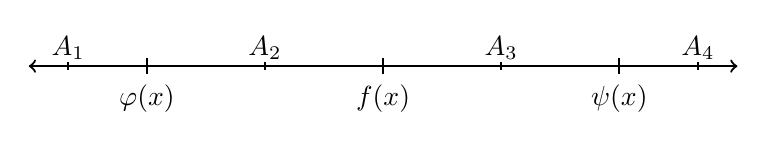
\begin{tikzpicture}[thick]
    \draw[thick, <->](0.5,0)--(9.5,0);
    \foreach \x/\xtext in {2/$\varphi(x)$, 5/$f(x)$, 8/$\psi(x)$}
      \draw(\x,3pt)--(\x,-3pt) node[below] {\xtext};
    \foreach \x/\xtext in {1/$A_1$, 3.5/$A_2$, 6.5/$A_3$, 9/$A_4$}
      \draw(\x, 1.5pt)--(\x,-1.5pt) node[above] {\xtext};
  \end{tikzpicture}
 \end{center}
  очевидно, что для любых допустимых взаимных расположений точек $A,\  \varphi(x),\  \psi(x),\  f(x)$ верно следующее неравенство:\newline
$(1)\quad |f(x) - A| \leq \max(|\varphi(x) - A|,\ |\psi(x) - a|)$\newline
Т.к. $\displaystyle \lim_{x \to a} \varphi(x) = \lim_{x \to a} \psi(x) = A$, то $\forall \varepsilon > 0$ существует $\varepsilon$-окрестность $U_a$ и\newline
$\varphi(x) \in U_{\varepsilon}(a)$ и $\psi(x) \in U_{\varepsilon}(a)$. Т.е. $|\varphi(x) - A| < \varepsilon$ и $|\psi(x) - A| < \varepsilon$.\newline
Тогда из (1) следует: $|f(x) - A| < \varepsilon$ из чего согласно определению предела по Коши следует, что $\displaystyle \lim_{x \to a} f(x) = A$, что и требовалось доказать.

\section{Доказательство эквивалентности определений по Коши и по Гейне}
\fixheader{Док-во равенства определений по}
\subsection{От Гейне к Коши}
Докажем от противного. Пусть $\displaystyle A = \lim_{x \to a} f(x)$ (по Гейне) и он не равен пределу по Коши. Т.е. (из определения по Коши):\newline
$\exists \varepsilon > 0:\ \forall \delta > 0:\ \exists x_{\delta} : \ 0<|x_{\delta} - a| < \delta$ и$\  |f(x_{\delta}) - A| \geq \varepsilon$ \newline
Рассмотрим $\delta = \frac{1}{n},\ $ где $ n \in \mathbb{N}$, обозначим последовательность значений в точке $\delta$ через $x_n$. Тогда имеем:\newline
$0 < |x_n - a| < \frac{1}{n}$, где $0 \to 0$ и $\frac{1}{n} \to 0$.
Из строгости неравенства следует $x_n \neq a$, а по теореме о трёх миллиционерах имеем:\newline
$|x_n - a| \to 0 \Rightarrow x_n \to a$, поэтому из определения по Гейне $f(x_n) \to A$, но по построению (т.к. $|f(x_{\delta}) - A| \geq \varepsilon$) $f(x_n) \not\to A$\newline\newline
Получили противоречие, значит если функция имеет предел по Гейне, то его можно определить и по Коши.

\subsection{От Коши к Гейне}
Пусть $\displaystyle A = \lim_{x \to a} f(x)$ по Коши. Т.е.\newline
$\displaystyle\ \forall \varepsilon > 0 : \ \exists \delta > 0: \ \forall x : \ 0 < |x - a| < \delta \ \Rightarrow \ |f(x) - A| < \varepsilon $\newline
Выберем произвольную последовательность  $x_n$  такую, что  $\displaystyle \lim_{n \to +\infty} x_n = a$. Т.к. $x_n$ стремится к $a$, то для любого $\delta$ > 0 найдется такой номер (обозначим его $n_\delta$), начиная с которго $\forall n>n_\delta$ будет выполнятся неравенство $|f(x_n) - A|<\varepsilon$, что по Коши равносильно $\displaystyle \lim_{n \to +\infty} f(x_n) = A$

\section{Теорема об единственности предела функции}
\fixheader{Т. об единственности предела ф-ции}
\begin{theorem}
$\begin{cases}\displaystyle \lim_{x \to a} f(x) = A_1 \\ \displaystyle \lim_{x \to a} f(x) = A_2\end{cases}$
$\Longrightarrow$ \qquad $\displaystyle A_1 = A_2$
\end{theorem}
Докажем от противного. Пусть $\displaystyle \lim_{x \to a} f(x) = A_1$ и $\displaystyle \lim_{x \to a} f(x) = A_2$\newline
Тогда из определения предела по Коши имеем $|f(x) - A_1| < \varepsilon$ и $|f(x) - A_2| < \varepsilon$.\newline 
Пусть $\varepsilon = \frac{\varepsilon_1}{2}$. Имеем:
\begin{center}$|f(x) - A_1| < \frac{\varepsilon_1}{2}$ и $|f(x) - A_2| < \frac{\varepsilon_1}{2}$.\end{center}
Рассмотрим выражение $|A_2 - A_1|$. Прибавим и отнимем $f(x)$:
\begin{center}$|A_2 - f(x) + f(x) - A_1|$\end{center}
Из свойств модуля следует:
\begin{center}$|A_2 - f(x) + f(x) - A_1| \leq |f(x) - A_1| + |f(x) - A_2|$\end{center}
Получаем:
\begin{center}$|A_2 - f(x) + f(x) - A_1| \leq |f(x) - A_1| + |f(x) - A_2| < \frac{\varepsilon_1}{2} + \frac{\varepsilon_1}{2}$, т.е. $|A_2 - A_1| < \varepsilon_1$\end{center}
Возьмём $\varepsilon_1 = |A_2 - A_1|$ и получим $|A_2 - A_1| < \frac{|A_2 - A_1|}{2}$. Противоречие. Значит предел функции единственный.

\section{Теорема о локальной ограниченности функции}
\fixheader{Т. о локальной огр. функции}
\begin{theorem}
Если функция имеет конечный предел при $x \to a$, то существует такая окрестность $a$, что функция на нём ограничена.
\begin{center}$\displaystyle \quad \lim_{x \to a} f(x) = A \Rightarrow \exists\  \mathring{U}(a),\  K > 0:\ \forall x \in \mathring{U}(a):\ |f(x)| \leq K$\end{center}
\end{theorem}
Из определения предела следует, что для любого положительного $\varepsilon$ существует $\delta > 0$ такая, что $\forall x \in \mathring{U_{\delta}}(a)\ |f(x) - A| < \varepsilon$. Из свойств модуля:
\begin{center}$A - \varepsilon < f(x) < A + \varepsilon$. Пусть $K = max(A - \varepsilon,\ A + \varepsilon)$\end{center} 
Тогда (опять же из свойств модуля) следует:\ $|f(x)| \leq K$, что и требовалось доказать.